\documentclass[11pt]{bgcletter}
\usepackage{url}
\usepackage{graphicx}

\newcommand{\answer}[1] {
{\color{cyan} #1}
}

\name{Dr.\ Carlos A. Sierra}
\signature{Carlos A. Sierra on behalf of all co-authors}
\email{csierra}
\telephone{8928}
\begin{document}
\begin{letter}{Editor\\
   Global Change Biology
}
\opening{Dear Editor,}
The reviewers were very positive about our revised version of the manuscript, and only suggested a few minor changes. 
In this new revised version, we address these comments, and in the text below we provide point-by-point \answer{answers} to each comment. 

As a summary, the main changes in this new version include:
\begin{itemize}
\item A new figure with an uncertainty analysis as requested by Reviewer 1. Although it was not possible to produce it for each specific biome due to unavailability of data at this level, this figure helps to reinforce some of the main arguments of the article.
\item To make space for this new figure, we combined previous figures 6 and 7 into a single figure (now Fig. 7). 
\item Small edits in the style of figures and corrections in text.
\end{itemize}

\textbf{Answers to reviewers' comments} \\
\textbf{Reviewer: 1}

Comments to the Author \\
This revised version has addressed most of my previous comments and the scope and quality of the manuscript have been improved. I particularly appreciate the new section on agroecosystem soil C. The manuscript is acceptable if the authors can address some remaining issues.

1. I still want to emphasize ``magnitude matters'', and the scattered information from numerical examples in sections 3.3 and 4.2 do not come together easily to benchmark one process vs another. A synthesis figure to quantitatively show the magnitude of major pathways in different biomes, either at the beginning of section 2 or after presenting numerical examples will be a memorable and highly citable contribution to the community by this review. I think the authors should spend some time to design that figure.

\answer{We added a new figure (new Fig 4) to the manuscript partially addressing the reviewer's comment (see below)}  

\begin{center}
   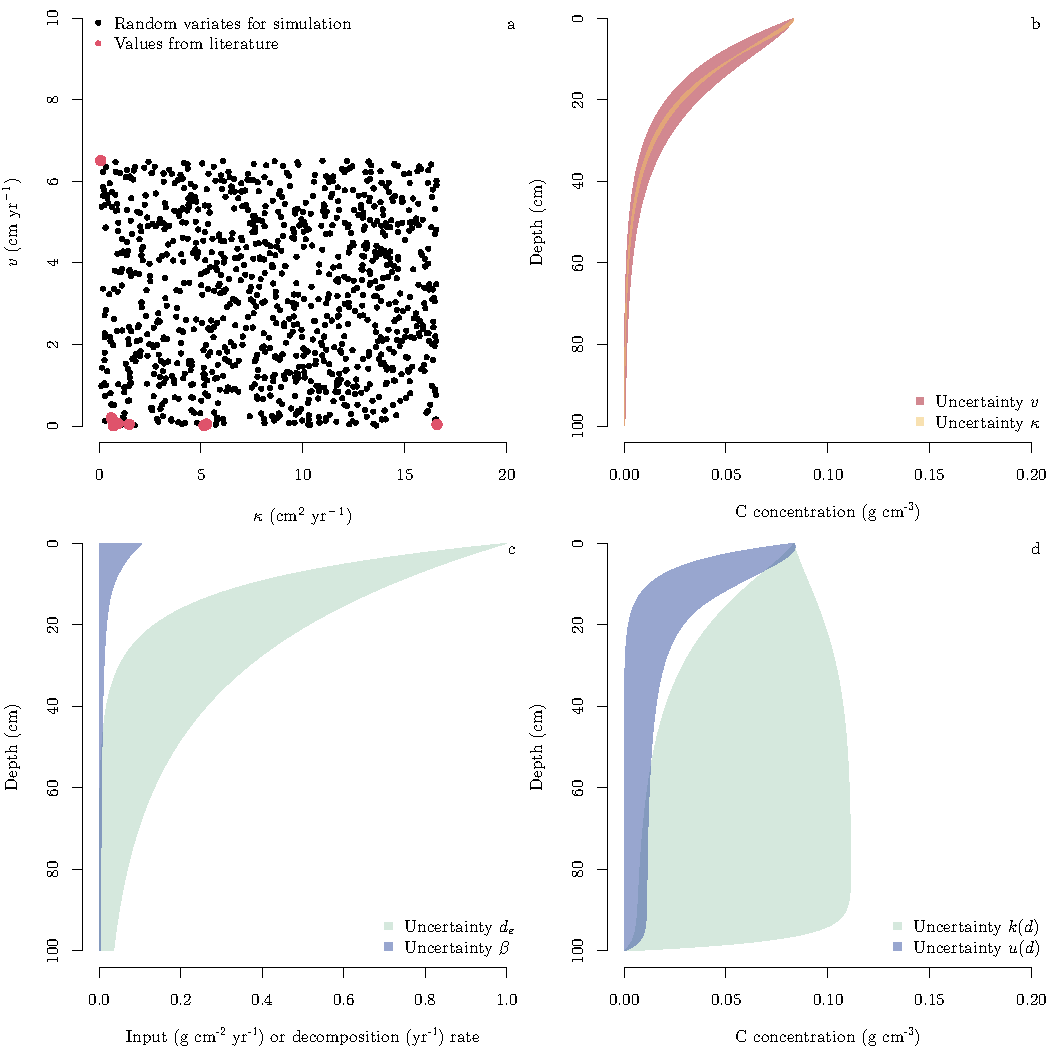
\includegraphics[width=\textwidth]{../Figures/uncertainty.pdf} \\
  \textit{\tiny Uncertainty analysis based on the components of equation 17 using a Monte Carlo uncertainty approach in which 1000 random variates of model parameters were chosen from a uniform distribution $U$. (a) Set of 1000 random variates of parameters $\kappa \sim U(0.09, 16.58)$ and $v \sim U(0.01, 6.51)$, and the set of values available from the literature (Table 1). (b) Prediction uncertainty in carbon concentration due to uncertainty in diffusion coefficient $\kappa$ and advection velocity $v$. (c) Uncertainty in the distribution of root inputs ($u(d)$) due to uncertainty in parameter $\beta \sim U(0.9, 1.0)$, and uncertainty in decomposition rate distribution ($k(d)$) due to uncertainty in parameter $d_e \sim U(10, 100)$. (d) Prediction uncertainty in carbon concentration due to uncertainty in root input distribution ($u(d)$) and decomposition rate distribution ($k(d)$). }
%   \label{fig:uncertainty}
\end{center}


\answer{We agree with the reviewer in that `magnitude matters' , and a conceptual figure showing the contribution of the different transport and decomposition processes for each biome would be an important contribution. We did spend a considerable amount of time thinking about such a figure, but unfortunately we came to the conclusion that the information currently available for each biome is not enough to produce such a figure. Although we were able to obtain values of transport coefficients $v$ and $\kappa$ for some sites and reported them in Table 1, this is not enough to derive biome-specific values for each coefficient. At the biome level, we do have information on belowground inputs, but without knowing how transport changes for each biome, we cannot make any meaningful predictions that would provide useful insights. On the contrary, we were worried that by producing a figure speculating about biome-specific values of $v$ and $\kappa$ we may send a misleading message. \\ The new figure we added presents an uncertainty analysis of the different components of equation 17, advection, diffusion, and vertical distribution of belowground inputs and decomposition. This figure addresses comment 3 below, and partially addresses this comment but not at the biome level. Instead the insights provided by this equation are general and are helpful to guide new research for specific biomes.  }

2. ``sum of the positive elements of x(t)''. The authors didn't get my point. I simply meant to suggest removing ``positive'', because when you say ``sum of the positive elements'', it indicates there are ``non-positive'' elements in x(t). \\
\answer{Done as suggested.}

3. The authors haven't directly addressed the overall uncertainty of equations in section 3.2. I agree with some of the justifications, but on the other hand would argue that parameter ranges in Table 1 and the uncertainties in different numerical examples are non-additive. This point connects to my previous suggestion for a synthesis figure to summarize different processes. Even results from a toy model help.

\answer{We included now an uncertainty analysis of the different components of equation 17 to show the relative importance of the difference processes on the prediction uncertainty of the vertical distribution of soil carbon. This uncertainty analysis reinforces one of the main messages of the article, root inputs and decomposition rate vertical distribution dominate the overall shape and uncertainty of the soil carbon profile, and dominate over transport processes. This new figure also partially addresses comment 1, but it was not possible to produce at the biome level due to unavailability of specific parameter values for each biome. }

%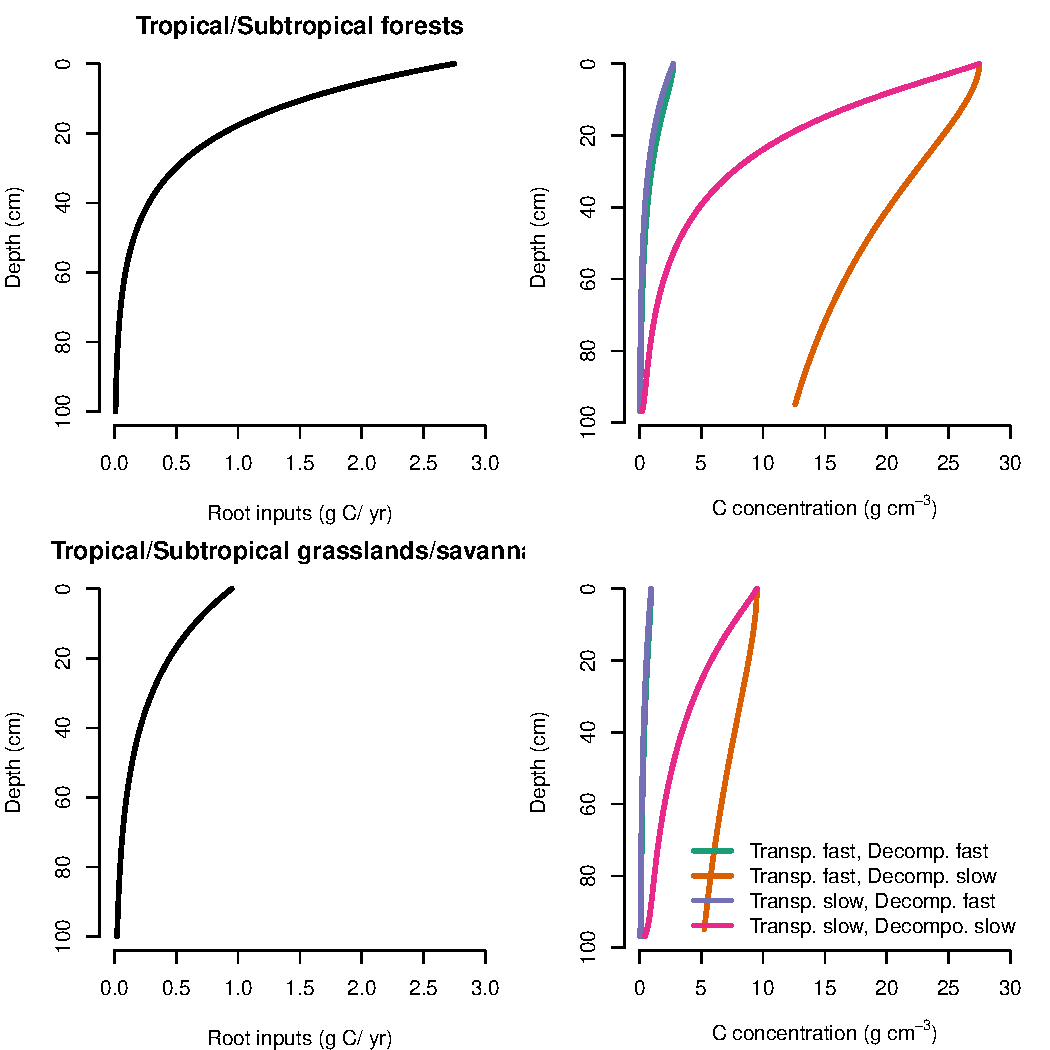
\includegraphics[scale=0.5]{exampleFig.pdf}

\newpage

\textbf{Reviewer: 2}

Comments to the Author \\
The manuscript has been improved based on reviewers’ comments. I thank the authors for their great effort. I only have minor suggestion.

Lines 19-21 “Land management activities could increase C storage in the subsoil by increasing advective vertical transport and decreasing the difference between inputs and decomposition at all depths.” This sentence seems contradicting to the previous sentence and to the main point of the manuscript. I think that the sentence in the main text “Conservation of existing subsoil C stocks seems to be a more relevant and important aspect because the timescales required to form existing soil C stocks were on the order of centuries to millenia and there are important risks that through land use change, or non-sustainable agricultural practices, important portions of these existing stocks may be lost quickly” is more consistent with the objective and an important message to the community. I would use it to end the abstract.

\answer{We removed this last sentence from the abstract as suggested by the reviewer.}

 \closing{Best regards,} 
% \encl{...}
% \cc{...}
% \ps{PS: Hope all is well.}
 \end{letter}

 \end{document}
